\section{DEZHA AIDIL MARTHA (1174025)}
\subsection{Pengertian}
Geografi adalah suatu ilmu yang mempelajari dan mendalami tentang lokasi suatu sistem peta, serta persamaan dan perbedaan variasi keruangan atas fenomena fisik, dan manusia di atas permukaan bumi. Geografi berasal dari Bahasa Yunani yaitu gêo "Bumi", dan graphein "Gambaran" atau "Menjelaskan". Para sarjana, praktisi, atau penulis di bidang Geografi disebut Geograf atau Geografer.Geografi juga merupakan nama judul buku bersejarah pada subjek ini, yang terkenal adalah Geographia tulisan Klaudios Ptolemaios pada abad-2.Geografi lebih dari sekadar kartografi, studi tentang peta. Geografi bukan hanya membahas apa, dan di mana di atas muka bumi, tapi juga mengapa sesuatu ada di situ, dan tidak di tempat lainnya, kadang bisa diartikan dengan "lokasi pada ruang." Geografi mempelajari hal ini, baik yang disebabkan oleh alam atau manusia. Juga mempelajari akibat yang disebabkan dari perbedaan yang terjadi itu.\hfill\break
Sistem informasi geografis (SIG) adalah sistem yang didesain untuk menangkap, menyimpan, mengolah, menganalisa, serta mempresentasikan data spasial.Dengan menghubungkan berbagai jenis data yang awalnya dianggap tidak berhubungan, SIG dapat membantu manusia dalam berbagai aspek pekerjaan. Proses menghubungkan ini umumnya dilakukan dalam konteks lokasi (spasial) dan waktu (temporal) yang sama.
\subsection{Sejarah}
Pada awalnya, peta hanya memiliki satu atau dua informasi saja didalamnya, sehingga jika seorang analis ingin mendapatkan informasi tambahan, dia harus melakukan overlay.Salah satu proses overlay pertama yang juga dianggap sebagai penerapan analisa spasial pertama secara sukses adalah oleh ilmuan / Geografer John Snow di London pada tahun 1854. Dia melakukan pemetaan terhadap lokasi orang-orang yang mengidap penyakit cholera dan menghubungkannya dengan peta penyediaan air minum London.\hfill\break
Pada awal abad ke-20, penggunaan teknik photozincography mulai meluas. Teknik ini memungkinkan peta terdiri dari beberapa layer yang nantinnya dapat diubah secara mandiri dari layer lainnya. Hal ini berguna untuk melakukan overlay dan analisa peta sesuai dengan layer yang dibutuhkan.Pada teknik ini, layer-layer yang ada dibuat dari film plastik atau lapisan kertas kalkir sehingga dapat digabungkan menjadi satu peta besar. Akan tetapi, teknik ini belum dapat dianggap sebagai SIG karena tidak terdapat database yang menghubungkan peta-peta tersebut.Pada tahun 1960, Canada mengembangkan sistem SIG pertamanya yang disebut CGIS atau Canada Geographic Information System. Sistem ini digunakan untuk menyimpan, mengolah, dan menganalisa informasi yang dimiliki oleh badan pertanahan Canada.
\subsection{Koordinat}
Koordinat didapatkan dari hasil perpotongan antara garis latitude (Y) / lintang dan garis longitude(X) / garis bujur sehingga bisa menunjukan suatu lokasi pada suatu daerah. \hfill\break 
Umumnya koordinat dibedakan menajadi koordinat Geografi dan Universal Transver Mercator(UTM). Pada koordinat geografi dibedakan menajadi 3 yaitu : \hfill\break
\begin{itemize}
	\item Degree, Decimal(DD, DDDD) contoh S 4.56734 E 102.67235
	\item Degree,Minute(DD MM,MMMM) contoh S 4 42,5423’ E 105 34,6445’
	\item Degree, Minute, Second(DD MM SS,SS) contoh : S 4 43’ 45,22 E 103 33’ 33,25
\end{itemize}
\hfill\break
\begin{figure}[H]
	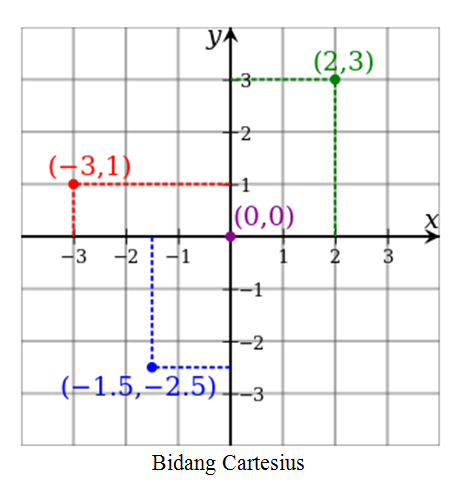
\includegraphics[width=4cm]{figures/1174025/1.png}
	\centering
	\caption{Contoh Koordinat}
\end{figure}
Pada system koordinat UTM biasanya terdapat pembagian waktu berdasarkan zonasinya. \hfill\break
\begin{figure}[H]
	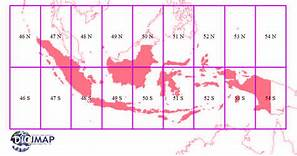
\includegraphics[width=4cm]{figures/1174025/2.jpg}
	\centering
	\caption{Contoh Koordinat UTM}
\end{figure}

\subsection{Data Geospasial}
Data geospasial merupakan pengambaran lokasi geografis,dimensi atau ukuran / karakteristik objek alam atau buatan manusia yang berada di bawah atau di atas permukaan bumi, data geospasial biasanya di singkat menjadi DG.
\hfill\break
Data Geospasial dibagi menjadi 3 yaitu :
\begin{itemize}
	\item Vektor
	Vektor merupakan salah jenis gambar yang dapat dibuat menggunakan aplikasi corel / adobe illustrator / aplikasi vektor lainnya. \hfill\break 
	Vektor itu sering digunakan untuk membuat gambar animasi dan vektor juga digunakan oleh goole maps.
	\item Roshen
	Roshen merupakan gambar yang di ambil dari satelit di luar angkasa, gambar ini biasanya bertipe jpg, dan pembaharuan data gambar ini berlangsung lama karena proses nya yang memakan waktu cukup banyak, jenis data ini digunakan oleh google earth.
	\item Roster
Data roster adalah data yang direpresentasikan dengan piksel dalam sebuah grafik. Data raster dihasilkan langsung oleh foto udara maupun foto satelit. Sehingga, secara umum, data roster lebih mudah dibuat dibandingkan dengan data vektor.
\end{itemize}

\subsection{Link}
\href{https://www.youtube.com/watch?v=Rw-D2J1h480}{Penjelasan GIT - Lalita Chandiany}
\subsection{Plagiarism}
\begin{figure}[H]
	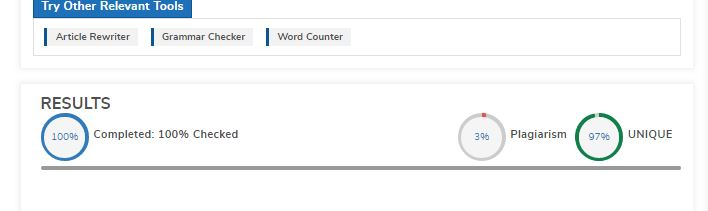
\includegraphics[width=4cm]{figures/1174025/plagiat.jpg}
	\centering
	\caption{Plagiat}
\end{figure}
